\chapter{Fondements théoriques:systémes et réseaux de neurones}

\section*{Introduction}

Ce chapitre présente les principes théoriques et conceptuels nécessaires pour comprendre ce travail. Il est divisé en deux parties complémentaires. La première partie concerne les principes généraux de la commande des systèmes. La deuxième partie concerne les réseaux de neurones artificiels et leur application à la commande des systèmes non linéaires. L'objectif principal de ce chapitre est de justifier le choix d'une approche neuronale pour la régulation thermique d'une enceinte, lorsque le modèle mathématique du système est inconnu ou difficile à identifier.

%=====================================================
\section{Généralités}
%=====================================================

L'automatique est la discipline de l'ingénieur qui répond à une
question fondamentale : comment faire en sorte qu'un système se
comporte comme on le souhaite ? Qu'il s'agisse de maintenir la
température d'un four, de stabiliser un drone en vol, ou de réguler
la vitesse d'un moteur, le problème est toujours le même : il faut
calculer une action de commande appropriée, en temps réel, malgré
les perturbations et les incertitudes.

La commande classique repose sur la connaissance d'un modèle mathématique du système. Ce modèle mathématique peut être une équation différentielle ou une fonction de transfert. Il décrit la relation entre l'entrée de commande, notée $u(t)$, et la sortie, notée $y(t)$. Une fois que ce modèle mathématique est identifié, il permet de prédire le comportement du système. Il permet également de concevoir une loi de commande adaptée au système.

L'outil central de cette démarche est le schéma fonctionnel, également appelé schéma-blocs. Le schéma fonctionnel représente graphiquement les interactions entre les différents composants du système.

%-----------------------------------------------------
\subsection{Représentation des systèmes}
%-----------------------------------------------------

On distingue deux grandes classes de systèmes selon le nombre de
leurs variables d'entrée et de sortie.

\begin{figure}[H]
	\centering
	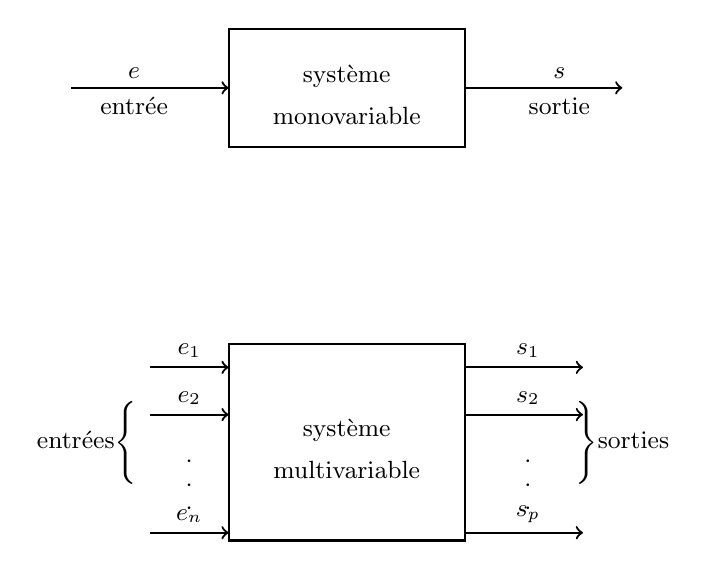
\begin{tikzpicture}
		
		%------------------------------------------
		% Système monovariable
		%------------------------------------------
		\draw[thick] (2, 0) rectangle (5, 1.5);
		\node[font=\small] at (3.5, 0.9) {système};
		\node[font=\small] at (3.5, 0.4) {monovariable};
		\draw[->, thick] (0, 0.75) -- (2, 0.75);
		\node[above, font=\small\itshape] at (0.8, 0.75) {$e$};
		\node[below, font=\small] at (0.8, 0.75) {entrée};
		\draw[->, thick] (5, 0.75) -- (7, 0.75);
		\node[above, font=\small\itshape] at (6.2, 0.75) {$s$};
		\node[below, font=\small] at (6.2, 0.75) {sortie};
		
		%------------------------------------------
		% Système multivariable
		%------------------------------------------
		\draw[thick] (2, -5) rectangle (5, -2.5);
		\node[font=\small] at (3.5, -3.6) {système};
		\node[font=\small] at (3.5, -4.1) {multivariable};
		\node[font=\small] at (0.2, -3.75) {entrées$\Bigg\{$};
		\draw[->, thick] (1.0, -2.8) -- (2, -2.8);
		\node[above, font=\small\itshape] at (1.5, -2.8) {$e_1$};
		\draw[->, thick] (1.0, -3.4) -- (2, -3.4);
		\node[above, font=\small\itshape] at (1.5, -3.4) {$e_2$};
		\node[font=\small] at (1.5, -4.0) {$\cdot$};
		\node[font=\small] at (1.5, -4.3) {$\cdot$};
		\node[font=\small] at (1.5, -4.6) {$\cdot$};
		\draw[->, thick] (1.0, -4.9) -- (2, -4.9);
		\node[above, font=\small\itshape] at (1.5, -4.9) {$e_n$};
		\draw[->, thick] (5, -2.8) -- (6.5, -2.8);
		\node[above, font=\small\itshape] at (5.8, -2.8) {$s_1$};
		\draw[->, thick] (5, -3.4) -- (6.5, -3.4);
		\node[above, font=\small\itshape] at (5.8, -3.4) {$s_2$};
		\node[font=\small] at (5.8, -4.0) {$\cdot$};
		\node[font=\small] at (5.8, -4.3) {$\cdot$};
		\node[font=\small] at (5.8, -4.6) {$\cdot$};
		\draw[->, thick] (5, -4.9) -- (6.5, -4.9);
		\node[above, font=\small\itshape] at (5.8, -4.9) {$s_p$};
		\node[font=\small] at (7.0, -3.75) {$\Bigg\}$sorties};
		
	\end{tikzpicture}
	\caption{Représentation des systèmes monovariable et multivariable.}
	\label{fig:mono_multi}
\end{figure}

Un \textbf{système monovariable} (SISO) possède une seule entrée et
une seule sortie, ce qui est le cas de l'enceinte thermique étudiée
dans ce travail : l'entrée est la puissance de chauffe $u(t)$ et la
sortie est la température $y(t)$. Un \textbf{système multivariable}
(MIMO) possède plusieurs entrées et plusieurs sorties, ce qui
complique significativement la synthèse de la loi de commande.

%-----------------------------------------------------
\subsection{Modèle d'un système}
%-----------------------------------------------------

Pour concevoir une loi de commande, il est indispensable de disposer
d'une représentation mathématique du système. On distingue deux
approches :

\begin{itemize}[label=$\bullet$]
	
	\item \textbf{Modèle de connaissance} : construit à partir des lois
	physiques (thermodynamique, mécanique, électromagnétisme).
	Il est précis mais souvent trop complexe pour être utilisé
	directement en commande, car il peut impliquer des équations
	aux dérivées partielles ou des paramètres difficiles à mesurer.
	
	\item \textbf{Modèle de commande} (ou modèle boîte noire) : obtenu à partir de mesures expérimentales grâce à une procédure d'identification. Les paramètres physiques
	n'apparaissent pas explicitement. Seule la relation
	entrée-sortie est modélisée. C'est cette approche qui est
	retenue dans ce travail.
\end{itemize}

%=====================================================
\section{Les réseaux de neurones artificiels}
%=====================================================

%-----------------------------------------------------
\subsection{Historique des réseaux de neurones artificiels}
%-----------------------------------------------------

L'histoire des réseaux de neurones artificiels est marquée par des avancées théoriques majeures.

\begin{itemize}[label=$\bullet$]
	
	\item \textbf{McCulloch et Pitts (1943)}
	e premier modèle mathématique du neurone biologique est celui du neurone formel \cite{[1]}. Ce modèle produit une sortie binaire. Cette sortie binaire est obtenue par seuillage d'une somme pondérée.
	\[
	y \;=\; \mathbf{1}_{\left\{ \sum_{i=1}^{n} w_i\,x_i \;\geq\; \theta \right\}}
	\]
	Ce modèle montre qu'un assemblage de neurones de cette façon peut réaliser n'importe quelle fonction logique.
	
	\item \textbf{Règle de Hebb (1949)}
	D. Hebb introduit le premier mécanisme d'apprentissage :
	deux neurones activés simultanément renforcent leur
	connexion synaptique :
	\[
	\Delta w_{ij} \;=\; \eta\; a_i\; a_j
	\]
	C'est le premier exemple d'apprentissage non supervisé.
	
	\item \textbf{Perceptron et Adaline (1958)}
	À cette époque, la notion du perceptron a été introduite. Le perceptron est le premier réseau à apprentissage supervisé. La règle de correction des poids du perceptron est proportionnelle à l'erreur de prédiction du perceptron.
	\[
	w_i \;=\; w_i + \eta\,(y - \hat{y})\,x_i
	\]
	Widrow et Hoff ont proposé en même temps l'\textbf{Adaline}.
	L'Adaline minimise l'erreur quadratique, notée $\mathcal{L}$, qui est égale à $\frac{1}{2}(y - \hat{y})^2$.
	Ceci est réalisé par la méthode de descente de gradient. L'Adaline constitue le modèle de base des réseaux multicouches.
	
	\item \textbf{Limites du Perceptron (Minsky et Papert, 1969)}
	Démonstration rigoureuse que le Perceptron ne résout que des problèmes linéairement séparables. En effet, il ne peut pas réaliser la fonction XOR :
	\[
	\nexists\;(w_1, w_2, \theta) \;\text{ tels que }\;
	w_1 x_1 + w_2 x_2 \geq \theta \iff x_1 \oplus x_2 = 1
	\]
	Cette démonstration provoque un premier hiver des réseaux
	de neurones.	
	\item \textbf{Cartes de Kohonen et machine de Boltzmann (1985)}
	Kohonen propose les cartes auto-organisatrices (apprentissage
	non supervisé). Hinton introduit la machine de Boltzmann,
	dont les états suivent une distribution de Gibbs-Boltzmann :
	\[
	P(\mathbf{s}) \;=\; \frac{1}{Z}\,
	e^{-E(\mathbf{s})/T}
	\]
	
	\item \textbf{1986 --- MLP et rétropropagation du gradient}
	Rumelhart, Hinton et Williams formalisent l'algorithme de
	\textbf{rétropropagation}, qui permet d'entraîner des réseaux
	multicouches. La propagation avant calcule :
	\[
	\mathbf{a}^{(\ell)} \;=\; f\!\left(
	\mathbf{W}^{(\ell)}\mathbf{a}^{(\ell-1)}
	+ \mathbf{b}^{(\ell)}\right)
	\]
	et la mise à jour des poids s'effectue par :
	\[
	\mathbf{W}^{(\ell)} \leftarrow \mathbf{W}^{(\ell)}
	- \eta\;\frac{\partial \mathcal{L}}
	{\partial \mathbf{W}^{(\ell)}}
	\]
	Le \textbf{théorème d'approximation universel} (Cybenko,
	1989) établit qu'un MLP à une couche cachée peut approximer
	toute fonction continue avec une précision arbitraire.
	
	\item \textbf{Jusqu'à aujourd'hui}
	Les réseaux de neurones profonds forment la base de l'intelligence artificielle moderne. Ils ont de nombreuses applications, notamment la commande de systèmes, le traitement du signal, la vision par ordinateur et l'analyse de séries temporelles. Les réseaux de neurones profonds sont vraiment très importants pour l'intelligence artificielle moderne.
	
\end{itemize}

%-----------------------------------------------------
\subsection{Commande neuronale d'un système inconnu}
%-----------------------------------------------------

Soit un système $(S)$ à entrée $u(t)$ et sortie $y(t)$ dont le
modèle mathématique est \textbf{inconnu}. L'objectif est de
générer $u(t)$ telle que $y(t)$ suive une consigne $r(t)$ :
\[
e(t) \;=\; r(t) - y(t) \;\longrightarrow\; 0
\]

\begin{itemize}[label=$\bullet$]
	
	\item \textbf{Approche classique} : un régulateur PID nécessite
	la connaissance explicite du modèle. Sans modèle,
	cette approche est inapplicable.
	
	\item \textbf{Approche neuronale} : le MLP joue deux rôles
	complémentaires.
	\begin{itemize}[label=$\circ$]
		\item \textbf{Identification} : un premier MLP apprend
		le comportement entrée-sortie du système :
		\[
		\hat{y}(t) = f_{\text{MLP}}\!\left(
		u(t),\, u(t-1),\, y(t-1),\, \ldots\right)
		\]
		\item \textbf{Commande} : un second MLP génère la
		commande en minimisant :
		\[
		\mathcal{L} \;=\; \frac{1}{N}\sum_{k=1}^{N}
		\bigl(r(t_k) - y(t_k)\bigr)^2
		\]
	\end{itemize}
	
\end{itemize}

\begin{figure}[H]
	\centering
	\begin{tikzpicture}[>=stealth, node distance=1.8cm,
		block/.style={rectangle, draw, thick, minimum width=2.2cm,
			minimum height=1cm, align=center},
		sum/.style={draw, thick, circle, minimum size=0.6cm,
			inner sep=0pt}]
		
		% Somme (soustracteur)
		\node[sum] (sum) {};
		
		% Contrôleur neuronal (MLP)
		\node[block, right=1.8cm of sum] (mlp) 
		{MLP \\ Contrôleur};
		
		% Système réel
		\node[block, right=1.8cm of mlp] (sys) 
		{Système réel};
		
		% Entrée de la consigne
		\draw[->] (sum.west) ++(-2,0) node[left] {$r$} -- (sum);
		\node[above left=0.08cm of sum] {$+$};
		\node[below left=0.08cm of sum] {$-$};
		
		% Signal d'erreur
		\draw[->] (sum) -- node[above] {$e$} (mlp);
		
		% Commande
		\draw[->] (mlp) -- node[above] {$u$} (sys);
		
		% Sortie du système
		\draw[->] (sys) -- ++(1.8,0) node[right] {$y$};
		
		% Boucle de retour (contre-réaction)
		\draw[->] ($(sys.east)+(0.6,0)$) coordinate (yfork)
		-- ++(0,-1.5) -| (sum.south);
		
	\end{tikzpicture}
	\caption{Structure de commande neuronale en boucle fermée. Le MLP joue le rôle du contrôleur neuronal direct.}
	\label{fig:commande_neuronale}
\end{figure}

La puissance de cette approche réside dans le fait que le MLP
apprend \textbf{implicitement} la dynamique du système à partir
des données d'entrée-sortie, sans modèle analytique explicite.

%-----------------------------------------------------
\subsection{Principes du MLP}
%-----------------------------------------------------

L'implémentation des réseaux de neurones artificiels repose sur deux principes :

\begin{itemize}[label=$\bullet$]
	
	\item \textbf{La mémoire informatique} : 
	
	Les paramètres du réseau ($\mathbf{W}^{(\ell)}$ et $\mathbf{b}^{(\ell)}$) sont stockés sous forme de tableaux de nombres réels. À chaque époque d'apprentissage, ces valeurs sont mises à jour et conservées. Cela permet l'accumulation progressive de l'information au fil du temps.
	
	\item \textbf{La méthode de résolution de l'analyse numérique} : La rétropropagation dans le calcul des paramètres du réseau implique des produits matriciels, l'évaluation de fonctions d'activation et le calcul de gradients. Tous ces éléments font partie de l'analyse numérique itérative.
	
\end{itemize}

%-----------------------------------------------------
\subsection{L'aspect mathématique du neurone artificiel}
%-----------------------------------------------------
Un neurone artificiel reçoit des entrées, qui sont notées $x_1, x_2, \ldots, x_n$. Chaque entrée a un poids synaptique, qui est noté $w_i$. Le neurone produit ensuite une sortie, qui est un nombre appelé $y$, et cela se fait en trois étapes.

\begin{figure}[H]
	\centering
	\begin{tikzpicture}[
		neuron/.style={circle, draw, minimum size=2.3cm, thick, fill=white},
		input/.style={inner sep=2pt, font=\large},
		arrow/.style={-Stealth, thick}]
		\node[neuron] (n) at (0,0) {};
		\draw[thick] (n.north) -- (n.south);
		\node at (-0.55,0) {$\displaystyle\sum_{i} w_i x_i$};
		\node at ( 0.55, 0) {$\varphi(\cdot)$};
		\node[input] (x1) at (-4, 1.2)  {$x_1$};
		\node[input] (x2) at (-4, 0)    {$x_2$};
		\node[input] (xn) at (-4,-1.2)  {$x_n$};
		\node at (-4,-0.5) {$\vdots$};
		\draw[arrow] (x1) -- node[above, pos=0.4]{$w_1$} (n.155);
		\draw[arrow] (x2) -- node[above, pos=0.4]{$w_2$} (n.180);
		\draw[arrow] (xn) -- node[above, pos=0.4]{$w_n$} (n.205);
		\node[input] (b) at (0,2) {$b$};
		\draw[arrow] (b) -- (n.90);
		\node[input] (y) at (3.5,0) {$y$};
		\draw[arrow] (n.0) -- (y);
		\node[left=3.8cm of n, font=\small, align=center]
		{Signaux\\d'entrée};
		\node[right=2.8cm of n, font=\small] {Sortie};
	\end{tikzpicture}
	\caption{Schéma structurel d'un neurone artificiel.}
\end{figure}

\paragraph{1. Pondération et sommation.}
\begin{equation}
	v \;=\; \sum_{i=0}^{n} w_i\,x_i
	\;=\; \mathbf{w}^\top \mathbf{x}
	\label{eq:potentiel}
\end{equation}
où $x_0 = 1$ et $w_0 = b$ (biais).

\paragraph{2. Activation.}
\begin{equation}
	y \;=\; f(v) \;=\; f\!\left(\mathbf{w}^\top \mathbf{x}\right)
	\label{eq:sortie_neurone}
\end{equation}

%-----------------------------------------------------
\subsection{Fonctions d'activation}
%-----------------------------------------------------

\paragraph{Fonction échelon (Heaviside).}
\begin{equation}
	f(v) \;=\; \begin{cases} 1 & v \geq \theta \\ 0 & \text{sinon}
	\end{cases}
\end{equation}
Non dérivable, elle est inadaptée à l'apprentissage par gradient.

\begin{figure}[H]
	\begin{center}
		\begin{tikzpicture}
			\begin{axis}[axis lines=middle, xlabel=$z$, ylabel={$g(z)$},
				xmin=-3, xmax=3, ymin=-0.2, ymax=1.2,
				ytick={0,1}, xtick={-2,0,2}, thick]
				\addplot[black, ultra thick, domain=-3:0] {0};
				\addplot[black, ultra thick, domain=0:3]  {1};
				\draw[dashed] (0,0) -- (0,1);
				\node[circle,draw,fill=white,inner sep=1.5pt] at (0,0) {};
				\node[circle,draw,fill=black,inner sep=1.5pt] at (0,1) {};
			\end{axis}
		\end{tikzpicture}
	\end{center}
	\caption{Fonction d'activation Heaviside.}
\end{figure}

\paragraph{Fonction linéaire.}
\begin{equation}
	f(v) \;=\; \alpha\,v, \qquad \alpha \in \mathbb{R}^+
\end{equation}
Utilisée en couche de sortie pour les problèmes de régression.

\paragraph{Fonction sigmoïde.}
\begin{equation}
	f(v) \;=\; \sigma(v) \;=\; \frac{1}{1 + e^{-v}},
	\qquad f(v) \in [0,\,1]
\end{equation}
Sa dérivée est :
\begin{equation}
	\sigma'(v) \;=\; \sigma(v)\,\bigl[1 - \sigma(v)\bigr]
\end{equation}

\begin{figure}[H]
	\begin{center}
		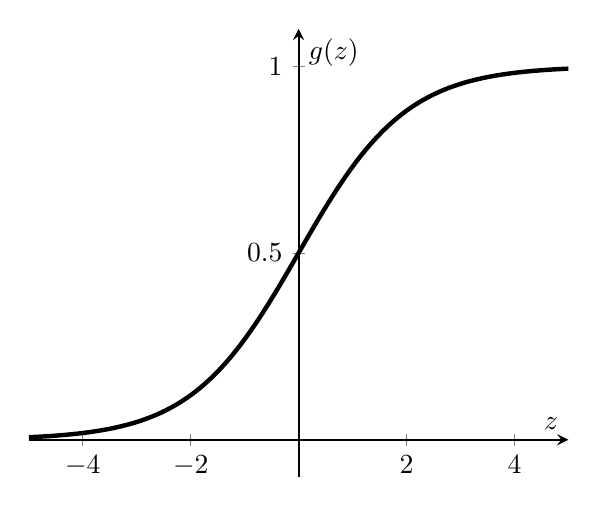
\begin{tikzpicture}
			\begin{axis}[axis lines=middle, xlabel=$z$, ylabel={$g(z)$},
				xmin=-5, xmax=5, ymin=-0.1, ymax=1.1,
				ytick={0,0.5,1}, thick]
				\addplot[black, ultra thick, domain=-5:5, samples=100]
				{1/(1+exp(-x))};
			\end{axis}
		\end{tikzpicture}
	\end{center}
	\caption{Graphique de la fonction d'activation sigmoïde.}
\end{figure}

\paragraph{Fonction tangente hyperbolique.}
\begin{equation}
	f(v) \;=\; \tanh(v) \;=\;
	\frac{e^{v} - e^{-v}}{e^{v} + e^{-v}},
	\qquad f(v) \in (-1,\,1)
\end{equation}
Sa dérivée est :
\begin{equation}
	\tanh'(v) \;=\; 1 - \tanh^2(v)
\end{equation}

\begin{figure}[H]
	\begin{center}
		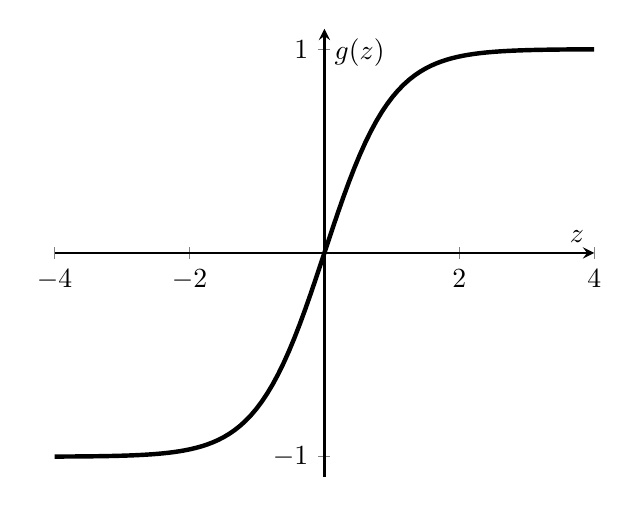
\begin{tikzpicture}
			\begin{axis}[axis lines=middle, xlabel=$z$, ylabel={$g(z)$},
				xmin=-4, xmax=4, ymin=-1.1, ymax=1.1,
				ytick={-1,0,1}, thick]
				\addplot[black, ultra thick, domain=-4:4, samples=100] {tanh(x)};
			\end{axis}
		\end{tikzpicture}
	\end{center}
	\caption{Graphique de la fonction d'activation tangente hyperbolique.}
\end{figure}

\subsection{Architecture du Perceptron Multi-Couche (MLP)}
%-----------------------------------------------------

Un MLP à $L$ couches cachées est constitué d'une couche d'entrée, de $L$ couches cachées et d'une couche de sortie.

Considérons un réseau à $L=4$ couches cachées, avec par exemple
$n_0=3$, $n_1=4$, $n_2=4$, $n_3=2$, $n_4=1$ neurones respectivement (soit 5 couches au total avec la couche d'entrée).

\begin{itemize}
	\item $n_\ell$ : nombre de neurones de la couche $\ell$. 
	Pour $\ell=1$, on a $n_1=4$ neurones dans la première couche cachée.
	
	\item $\mathbf{W}^{(\ell)} \in \mathbb{R}^{n_\ell \times n_{\ell-1}}$ :
	matrice des poids de la couche $\ell$. Pour $\ell=1$, elle relie
	les $n_0=3$ entrées aux $n_1=4$ neurones :
	\[
	\mathbf{W}^{(1)} \in \mathbb{R}^{4 \times 3}
	\;=\;
	\begin{pmatrix}
		w^{(1)}_{11} & w^{(1)}_{12} & w^{(1)}_{13} \\
		w^{(1)}_{21} & w^{(1)}_{22} & w^{(1)}_{23} \\
		w^{(1)}_{31} & w^{(1)}_{32} & w^{(1)}_{33} \\
		w^{(1)}_{41} & w^{(1)}_{42} & w^{(1)}_{43}
	\end{pmatrix}
	\]
	
	\item $\mathbf{b}^{(\ell)} \in \mathbb{R}^{n_\ell}$ : vecteur des biais
	de la couche $\ell$. Pour $\ell=1$ :
	\[
	\mathbf{b}^{(1)} =
	\bigl[b^{(1)}_1,\; b^{(1)}_2,\; b^{(1)}_3,\; b^{(1)}_4\bigr]^\top
	\in \mathbb{R}^{4}
	\]
	
	\item $\mathbf{a}^{(\ell)} \in \mathbb{R}^{n_\ell}$ : vecteur des
	activations de la couche $\ell$. Pour $\ell=1$ :
	\[
	\mathbf{a}^{(1)} =
	\bigl[a^{(1)}_1,\; a^{(1)}_2,\; a^{(1)}_3,\; a^{(1)}_4\bigr]^\top
	\in \mathbb{R}^{4}
	\]
	et la relation de propagation s'écrit :
	\[
	\mathbf{a}^{(\ell)} = \varphi\!\left(\mathbf{W}^{(\ell)}\,
	\mathbf{a}^{(\ell-1)} + \mathbf{b}^{(\ell)}\right),
	\quad \ell = 1,2,3,4
	\]
	avec $\mathbf{a}^{(0)} = \mathbf{x}$ le vecteur d'entrée.
	
\end{itemize}

\begin{figure}[H]
	\centering
	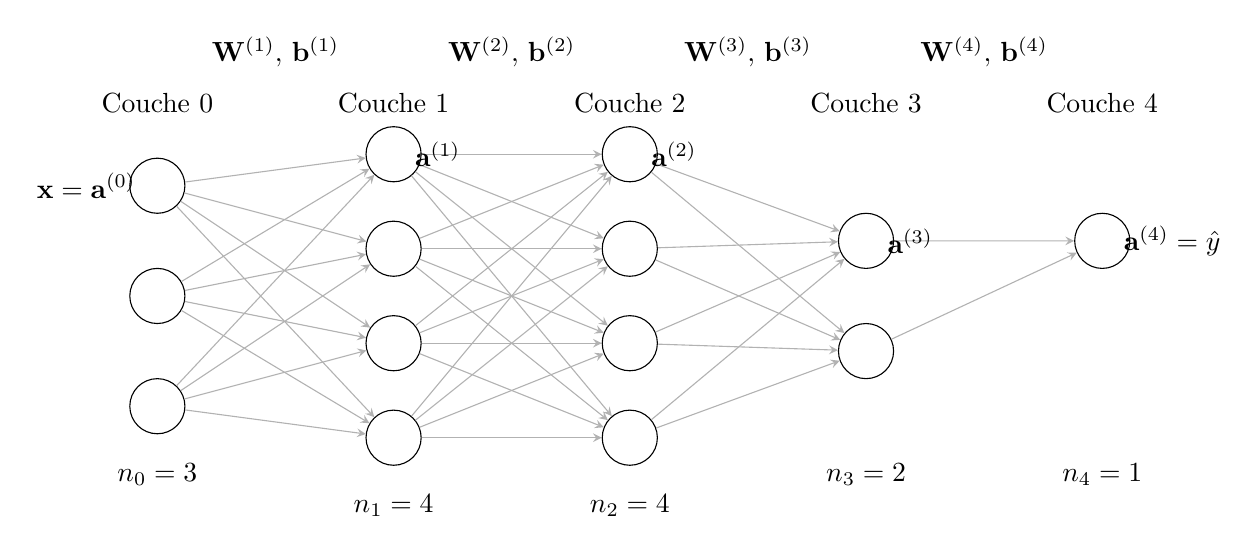
\begin{tikzpicture}[
		neuron/.style={circle, draw=black, fill=white,
			minimum size=0.7cm, inner sep=0pt},
		>=stealth]
		
		% Couche 0 : entrée (3 neurones)
		\foreach \i in {1,2,3}{
			\node[neuron] (I\i) at (0,-\i*1.4) {};}
		\node[above] at (0,-0.6)  {Couche $0$};
		\node[below] at (0,-4.8)  {$n_0=3$};
		
		% Couche 1 : première couche cachée (4 neurones)
		\foreach \i in {1,2,3,4}{
			\node[neuron] (H1\i) at (3,-\i*1.2+0.2) {};}
		\node[above] at (3,-0.6)  {Couche $1$};
		\node[below] at (3,-5.2)  {$n_1=4$};
		
		% Couche 2 : deuxième couche cachée (4 neurones)
		\foreach \i in {1,2,3,4}{
			\node[neuron] (H2\i) at (6,-\i*1.2+0.2) {};}
		\node[above] at (6,-0.6)  {Couche $2$};
		\node[below] at (6,-5.2)  {$n_2=4$};
		
		% Couche 3 : troisième couche cachée (2 neurones)
		\foreach \i in {1,2}{
			\node[neuron] (H3\i) at (9,-\i*1.4-0.7) {};}
		\node[above] at (9,-0.6)  {Couche $3$};
		\node[below] at (9,-4.8)  {$n_3=2$};
		
		% Couche 4 : sortie (1 neurone)
		\node[neuron] (O1) at (12,-2.1) {};
		\node[above] at (12,-0.6) {Couche $4$};
		\node[below] at (12,-4.8) {$n_4=1$};
		
		% Connexions 0 -> 1
		\foreach \i in {1,2,3} \foreach \j in {1,2,3,4}
		\draw[->, gray!60, thin] (I\i) -- (H1\j);
		
		% Connexions 1 -> 2
		\foreach \i in {1,2,3,4} \foreach \j in {1,2,3,4}
		\draw[->, gray!60, thin] (H1\i) -- (H2\j);
		
		% Connexions 2 -> 3
		\foreach \i in {1,2,3,4} \foreach \j in {1,2}
		\draw[->, gray!60, thin] (H2\i) -- (H3\j);
		
		% Connexions 3 -> 4
		\foreach \i in {1,2}
		\draw[->, gray!60, thin] (H3\i) -- (O1);
		
		% Etiquettes des matrices
		\node at (1.5, 0.3) {$\mathbf{W}^{(1)},\,\mathbf{b}^{(1)}$};
		\node at (4.5, 0.3) {$\mathbf{W}^{(2)},\,\mathbf{b}^{(2)}$};
		\node at (7.5, 0.3) {$\mathbf{W}^{(3)},\,\mathbf{b}^{(3)}$};
		\node at (10.5,0.3) {$\mathbf{W}^{(4)},\,\mathbf{b}^{(4)}$};
		
		% Etiquettes des vecteurs d'activation
		\node[left=0.15cm]  at (I1)   {$\mathbf{x}=\mathbf{a}^{(0)}$};
		\node[right=0.15cm] at (H11)  {$\mathbf{a}^{(1)}$};
		\node[right=0.15cm] at (H21)  {$\mathbf{a}^{(2)}$};
		\node[right=0.15cm] at (H31)  {$\mathbf{a}^{(3)}$};
		\node[right=0.15cm] at (O1)   {$\mathbf{a}^{(4)}=\hat{y}$};
		
	\end{tikzpicture}
	\caption{Architecture d'un MLP à $L=4$ couches cachées
		($n_0=3,\;n_1=4,\;n_2=4,\;n_3=2,\;n_4=1$).}
	\label{fig:mlp_exemple}
\end{figure}

\paragraph{Propagation avant (\textit{forward pass}).}
Pour $\ell = 1, \ldots, L$ :
\begin{align}
	\mathbf{z}^{(\ell)} &\;=\;
	\mathbf{W}^{(\ell)}\,\mathbf{a}^{(\ell-1)} + \mathbf{b}^{(\ell)}
	\label{eq:preactivation} \\[4pt]
	\mathbf{a}^{(\ell)} &\;=\;
	f^{(\ell)}\!\left(\mathbf{z}^{(\ell)}\right)
	\label{eq:activation_vect}
\end{align}
avec $\mathbf{a}^{(0)} = \mathbf{x}$ et
$\hat{\mathbf{y}} = \mathbf{a}^{(L)}$.

\paragraph{Réseaux de neurones à une couche cachée ($L = 2$ couches cachées au sens strict, mais ici on note $L=3$ couches totales)}
Pour $n$ entrées du réseau, $q$ neurones de la couche cachée et une seule sortie :
\begin{equation}
	\hat{y} \;=\; \sum_{j=1}^{q} w_j^{(2)}\,
	\tanh\!\left( b_j^{(1)}
	+ \sum_{i=1}^{n} w_{ji}^{(1)}\,x_i \right)
	+ b^{(2)}
	\label{eq:PMC_scalaire}
\end{equation}

%-----------------------------------------------------
\subsection{Apprentissage par rétropropagation du gradient}
%-----------------------------------------------------

\subsubsection*{Fonction de coût et problème de minimisation}

L'objectif de l'apprentissage est de trouver les paramètres optimaux 
$\boldsymbol{\theta} = \{\mathbf{W}^{(\ell)},\, \mathbf{b}^{(\ell)}\}$
qui minimisent l'erreur quadratique moyenne :
\begin{equation}
	\mathcal{L}(\boldsymbol{\theta}) \;=\;
	\frac{1}{N}\sum_{k=1}^{N}
	\left\| \mathbf{y}^{(k)} - \hat{\mathbf{y}}^{(k)} \right\|^2
	\label{eq:MSE}
\end{equation}
où $\hat{\mathbf{y}}^{(k)}$ est la sortie du réseau pour le $k$-ième exemple,
obtenue par propagation avant successive :
\begin{equation}
	\hat{\mathbf{y}}^{(k)} = \mathbf{a}^{(L,k)}, \qquad
	\mathbf{a}^{(\ell,k)} = \varphi\!\left(
	\mathbf{W}^{(\ell)}\,\mathbf{a}^{(\ell-1,k)} + \mathbf{b}^{(\ell)}
	\right), \quad \ell = 1,\ldots,L
	\label{eq:forward}
\end{equation}
avec $\mathbf{a}^{(0,k)} = \mathbf{x}^{(k)}$ le vecteur d'entrée,
soit trouver :
\[
\boldsymbol{\theta}^* \;=\; \arg\min_{\boldsymbol{\theta}}\;
\mathcal{L}(\boldsymbol{\theta})
\]

\subsubsection*{Pourquoi la descente de gradient ?}

Il y a deux méthodes de résolution mathématique pour minimiser 
$\mathcal{L}(\boldsymbol{\theta})$ :

\begin{itemize}[label=$\bullet$]
	
	\item \textbf{Solution analytique} : celle de l'algèbre linéaire qui consiste à annuler les dérivées partielles
	$\frac{\partial \mathcal{L}}{\partial \boldsymbol{\theta}} = 0$
	conduit à l'inversion d'une matrice de taille $D \times D$,
	de complexité $\mathcal{O}(D^3)$. Pour un réseau avec des
	milliers de paramètres, cette opération est
	\textbf{numériquement prohibitive}.
	
	\item \textbf{Descente de gradient de l'analyse numérique} : qui consiste à corriger itérativement les
	paramètres du réseau dans le sens opposé au gradient :
	\[
	\boldsymbol{\theta} \;\leftarrow\;
	\boldsymbol{\theta} - \eta\,
	\nabla_{\boldsymbol{\theta}}\,\mathcal{L}
	\]
	La complexité de chaque itération est $\mathcal{O}(ND)$. Puisque $\mathcal{L}$ 
	est convexe, la convergence vers le minimum global est garantie.
	
\end{itemize}

\subsubsection*{Algorithme de rétropropagation}

Dans le cas d'un neurone unique ($L=1$, $n_0=3$, $n_1=1$),
le réseau se réduit à :
\[
\hat{y} = \varphi\!\left(w_1 x_1 + w_2 x_2 + w_3 x_3 + b\right)
\]
où $w_1, w_2, w_3 \in \mathbb{R}$ sont les poids et $b \in \mathbb{R}$ le biais.

\paragraph{Étape 1 : Signal d'erreur en sortie.}
\begin{equation}
	\delta = \bigl(\hat{y} - y\bigr)\cdot\varphi'(z) \;\in\; \mathbb{R}
\end{equation}
où $z = w_1 x_1 + w_2 x_2 + w_3 x_3 + b \in \mathbb{R}$.

\paragraph{Étape 2 : Mise à jour des paramètres.}
\begin{align}
	w_1 &\leftarrow w_1 - \eta\;\delta\; x_1 \notag\\
	w_2 &\leftarrow w_2 - \eta\;\delta\; x_2 \notag\\
	w_3 &\leftarrow w_3 - \eta\;\delta\; x_3 \notag\\
	b   &\leftarrow b   - \eta\;\delta          \notag
\end{align}
Ces deux étapes sont répétées sur l'ensemble des données jusqu'à
convergence de $\mathcal{L}$ vers son minimum.

%-----------------------------------------------------
\subsection{Le modèle récursif général du MLP}
%-----------------------------------------------------

De façon générale, un MLP à $L+2$ couches peut s'écrire
récursivement :
\[
x_{\ell+1} \;=\;
\begin{cases}
	g(\theta_\ell\, x_\ell) & \ell = 0, 1, \ldots, L-1 \\
	f(\theta_L\, x_L)       & \ell = L
\end{cases}
\]
où $\theta_\ell = (b_\ell \mid W_\ell)$ est la matrice de poids
partitionnée ($W_\ell \in \mathbb{R}^{n_{\ell+1} \times n_\ell}$,
$b_\ell \in \mathbb{R}^{n_{\ell+1}}$), $x_0$ est le vecteur
d'entrée, $x_{L+1}$ la sortie, et $g$, $f$ sont respectivement
les fonctions d'activation des couches cachées et de la couche
de sortie.

%=====================================================
\section*{Conclusion}
%=====================================================

Ce premier chapitre a présenté les éléments essentiels pour comprendre le travail. Les principes de base de la commande en boucle fermée ont été définis, en incluant la définition des critères de performance importants — la précision, la rapidité et la stabilité — qui sont les principaux défis à relever lors de la création d'un régulateur.

Le régulateur PID, dont la loi de commande :
\[
u(t) \;=\; K_p\,e(t)
+ K_i\int_{0}^{t} e(\tau)\,\mathrm{d}\tau
+ K_d\,\frac{\mathrm{d}e(t)}{\mathrm{d}t}
\]
offre un compromis éprouvé depuis plus d'un siècle. Cependant,
ses performances sont conditionnées par la connaissance du modèle
mathématique du système, ce qui constitue une limitation majeure
face aux systèmes non linéaires ou mal connus.

C'est pour répondre à cette limitation que les réseaux de neurones
artificiels ont été introduits. Le MLP, dont l'apprentissage par
rétropropagation minimise :
\[
\mathcal{L}(\boldsymbol{\theta}) \;=\;
\frac{1}{N}\sum_{k=1}^{N}
\left\| \mathbf{y}^{(k)} - \hat{\mathbf{y}}^{(k)} \right\|^2
\]
est capable d'identifier implicitement la dynamique d'un système
inconnu à partir de ses seules données d'entrée-sortie.

Fort de ces bases, le chapitre suivant présente les simulations
réalisées pour valider ces deux approches sur des systèmes
linéaires et non linéaires, avant leur application expérimentale
à la régulation thermique de l'enceinte.